
\section{Introduction}\index{Introduction}

The purpose of a particle physics detector is to find all the particles produced
in a collision, identify their types, and measure their 4-momenta.
At the LHC, in a single collision, thousands of particles can be produced.
The particle physics detector must make signals that somehow can yield this information.
To understand how this can happen, we first must understand how particles interact
with matter, so we can learn of the possible types of signals particles can produce.

What kinds of particles can an LHC detector detect?  First, the particle must live long 
enough to reach the detector without decaying.  The beam pipe of the LHC has a 
radius with dimensions measured in cm.  The particle must exist long enough to escape the beam pipe and
reach the detector and make a signal.  If we take the diameter to be 1 cm, then
the particle life time must be large enough to travel this far before decay.
How far does a particle travel before decaying?  We learned in Chapter \ref{EP} that fraction remaining after a time $t_0$ is given by
\begin{equation}
N=N_0 e^{-t_0 \over \tau}
\end{equation}
The probability of surviving is $N / N_0$ so
\begin{equation}
P(t)= e^{-t_0 \over \tau}
\end{equation}
To change this to the probability of traveling a distance instead of a time, remember that that, with relativity, the life time for a moving particle depends on the lifetime for the particle at rest as $\tau = \gamma \tau_0$ so we have
 \begin{equation}
P(t)=e^{-t_0 \over {\gamma \tau_0}}
\end{equation}
Position is then related to time by $x_0=vt_0$ or $x_0=\beta c t_0$, so
\begin{equation}
P(t)=e^{-x_0 \over {\beta c \gamma \tau_0}}
\end{equation}
Then, using
$\Gamma=\bar{h}/\tau_0$, $\gamma=E/mc^2$ where m is the particle's mass 
and $\beta=pc/E$, we have
\begin{equation}
P(x_0)=e^{{-x_0\Gamma mc^2}\over{pc\bar{h}c}}
\end{equation}

The particle must also interact  with matter in a way that produces a large enough signal to measure in a detector that is small enough to be affordable.  While specialized very large detectors exist which can detect neutrinos, this is not possible at a collider detector.

There are only a few types of particles (and their antiparticles) that satisfy these requirements, and they are:  From the leptons: electrons and muons; From the bosons: photons; From the mesons:
charged pions, charged kaons (remember: these contain a strange quark), k-longs (a type of rare kaon; kaons, as you remember are mesons containing a strange quark); From the baryons: protons, neutrons.

The most common particle produced in a proton-proton collision is the pion.  Neutral pions decay very quickly to two photons. Most of the particles we detect, therefore, will be charged pions and photons.  However, as we will discuss, particles like electrons and muons are signatures of Higgs decays, and so we need to have a detector well optimized for identifying and measuring these particles as well.




\section{Interactions of charged particles with matter}\index{chargedinteractions}
We will first look at possible signals from charged particles (electrons, muons, charged pions, protons).

Possible interactions between these particles and bulk matter include:
\begin{itemize}
\item ionization and excitation of the molecules in the material
\item multiple scattering
\item bremsstrahlung
\item strong interactions with atomic nucleii (only for mesons and baryons, as these contain quarks)
\end{itemize}
We will postphone the discussion of the last two of these interactions until our discussion of ``calorimetry''.

When a charged particle passes through some material (detectors are often made of Argon gas, silicon, iron, lead, steel, plastic, and other such materials), it will interact with the electrons in the molecules that make up that material via the electric force.  
The charged particle loses energy as it passes through the material, and the material gains energy.  
It is somewhat similar to sliding friction.  For example, when a book slides across a table, the molecules in the book interact with those on the table via the electric force.  This causes the kinetic energy of the book to leave it, and become heat energy in the book and the table.  This heat energy, you may remember, is associated with the random, invisible motion of the molecules in the book and table.  There is a difference though.  The energy of the charged particle doesn't initially produce heat (although, eventually, some heating can occur.)
What effect does that energy have on the material?  It can cause the electrons in the material to ``be excited'' into higher quantum states or it can even detach an electron from its atom (``ionization'').  This excitation energy can eventually turn into heat energy or it can produce signals that can be detected, as we will discuss later.

We are often interested in how much energy the particle loses (material gains) per unit length.  This is called $dE/dx$, pronounced ``d-E-d-x''.    The average amount of energy lost per unit length depends on the energy of the particle: low energy particles lose more energy per unit length than high energy particles.  You can imagine why this might be true: the lower energy (slower) particles linger near each atom in the materi[al longer, and thus have a longer time to interact with each one and lose more energy.  The energy loss per unit length decreases as $1/\beta^2$ until a momentum around 0.1 GeV, where it has its minimum value.  The loss then increases slowly with increasing energy until about 100 GeV.  Above this energy, relativistic effects cause dEdx to increase more quickly with energy.  Particles in the momentum range of 0.1 to 100 GeV are called "minimum ionizing particles" or "mips".

Figure ~\ref{fig:pdgdedx} shows the energy dependence of dEdx for various charged particles.  Note that the length unit is strange: it is $cm^2/g$.  You can convert this to a more convention length unit by multiplying by the density of the material
\begin{equation}
{{MeV cm^2}\over{g}} \cdot {{g}\over{cm^3}} = {{MeV}\over{cm}}
\end{equation}
The reason the authors use these units is that it allows the dEdx curves for high Z and low Z elements to fit onto the same graph.

\begin{figure}[h]
\centering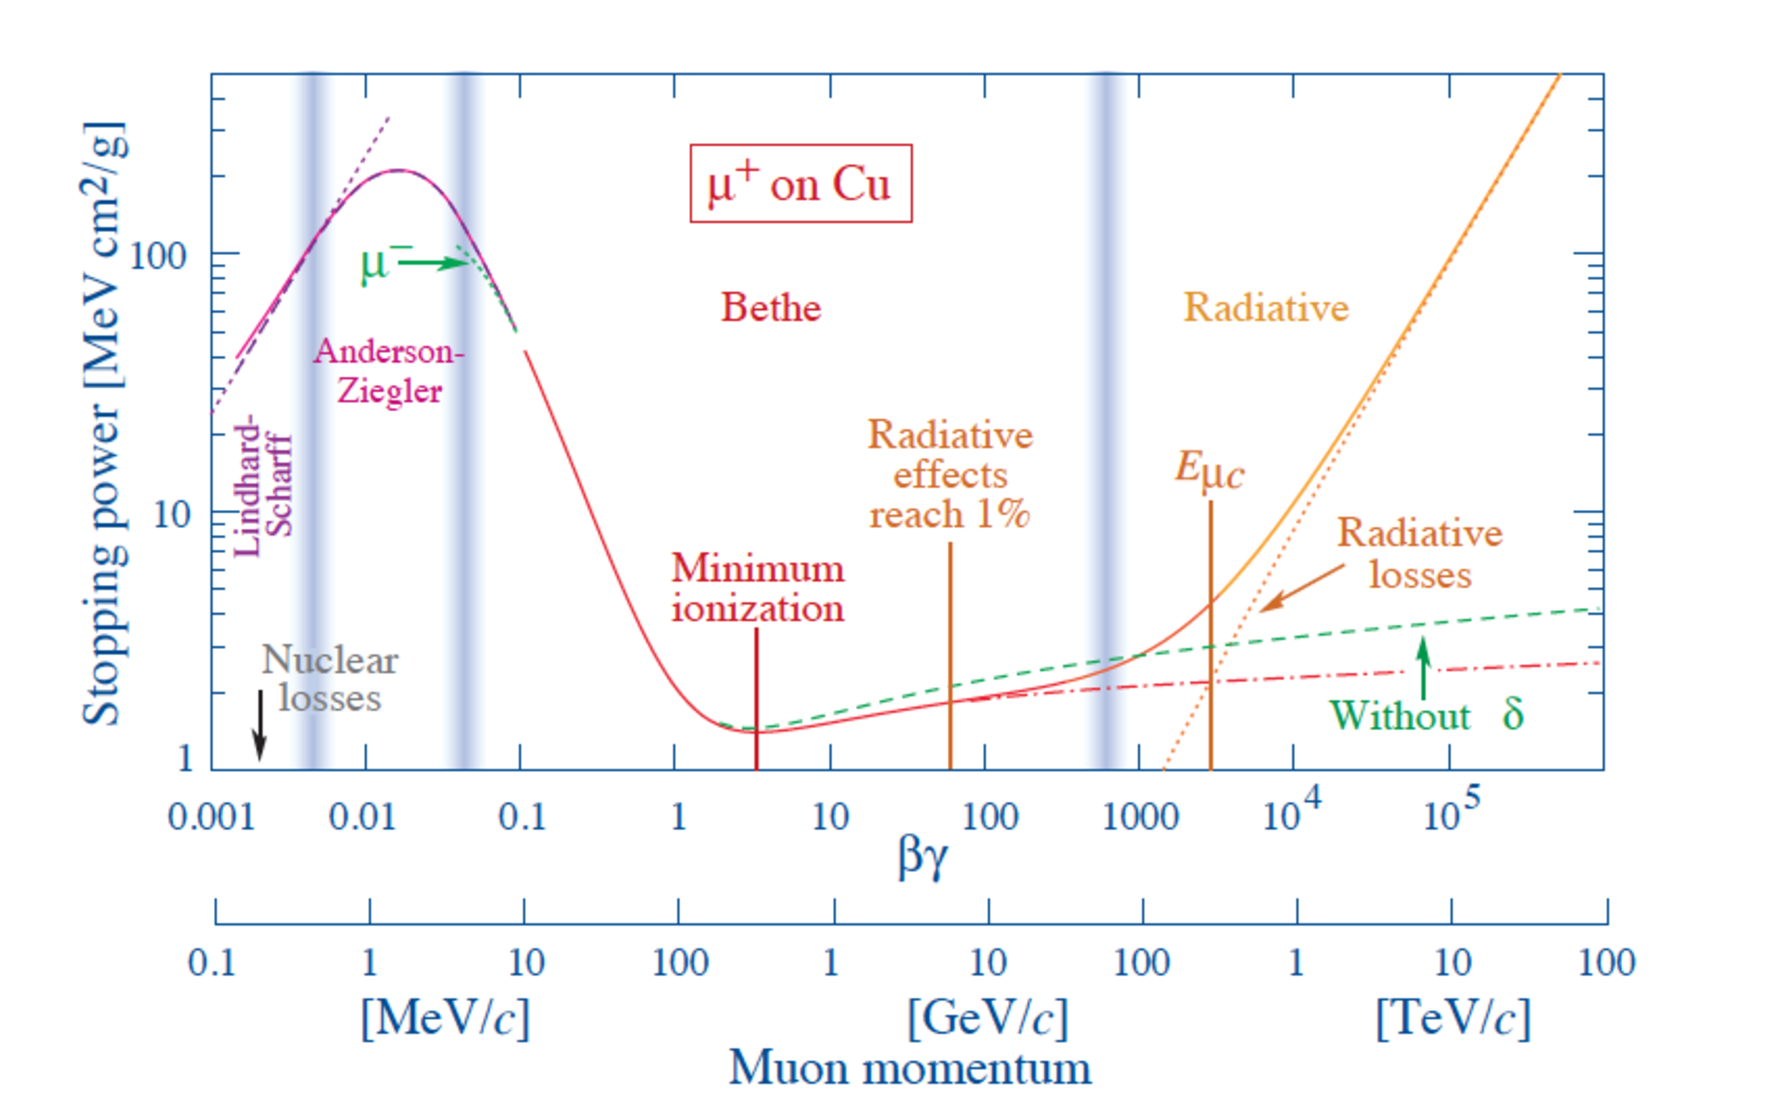
\includegraphics[scale=0.5]{./particleinteractions/Pictures/dedx.pdf}
\caption{Stolen from the particle data group, this picture shows the energy
loss per unit length as a function of particle energy}
\label{fig:pdgdedx}
\end{figure}

What kind of signals can be produced this way?  If the material is a gas, the electrons produced through ionization can be gathered on a wire (using an electric field produced by voltages on metal pads on the structure holding the gas or on wires running through the gas) to produce a current.  The signals from silicon are similar.  If the material is a plastic scintilator, some of the ``excited'' molecules will ``de-excite'' by emitting photons, which can be detected with a photomulitplier tube or other light sensitive device.

If the material is thick and high-Z (iron, lead), the particle may lose all its energy and 
stop inside the material.  The thickness of material that will stop a particle (of a given energy) is called the particle's range.  Fig~\ref{fig:pdgrange} shows the range for various particles in various materials as a function of particle energy.


\begin{figure}[h]
\centering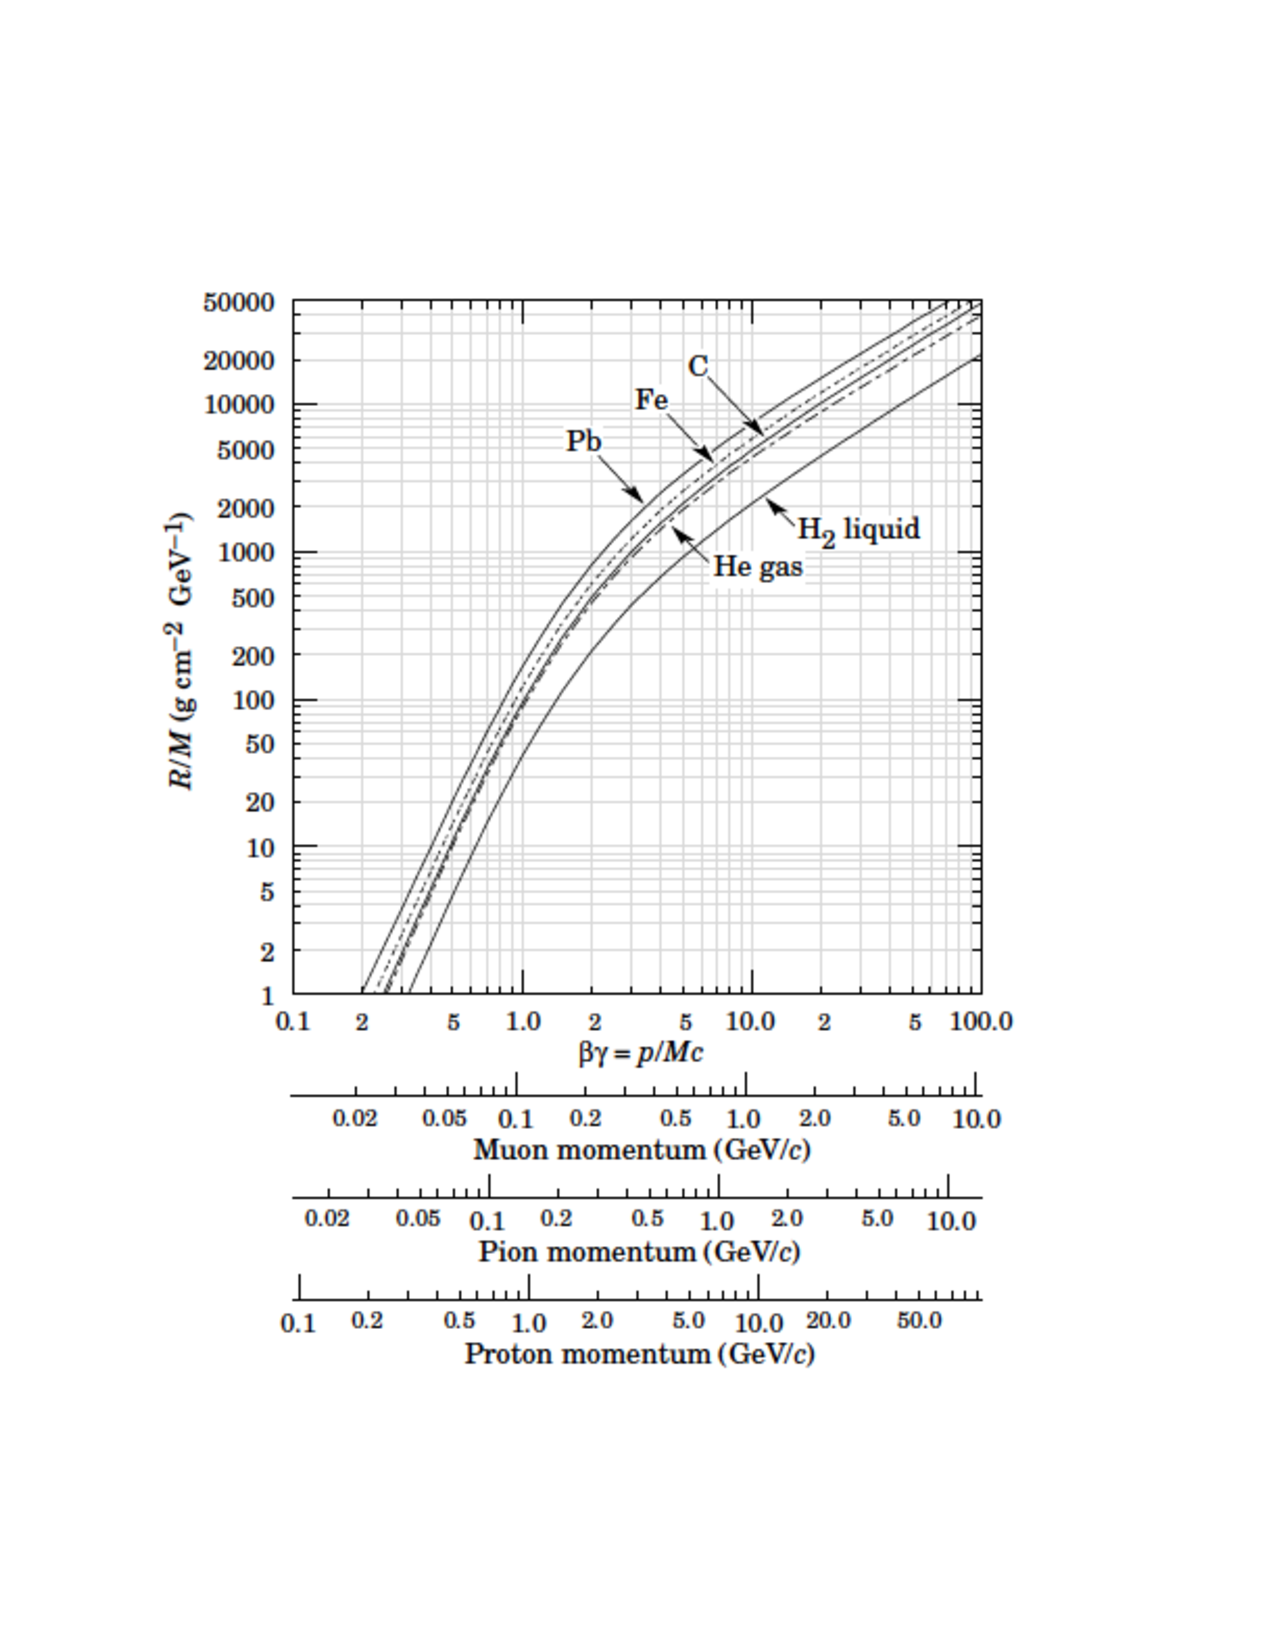
\includegraphics[scale=0.5]{./particleinteractions/Pictures/pdgrange.pdf}
\caption{Stolen from the particle data group, this picture shows the range of a particle in various materials as a function of particle energy }
\label{fig:pdgrange}
\end{figure}

Of course, because each particle that goes through the material will randomly interact with different numbers of atomic electrons, exchanging more energy when it happens to go close to one, and exchanging less when it is further away, particle by particle the amount of energy varies.  The disttribution of deposted energies follows a "Landau" distribution, as shown in Fig~\ref{fig:landau}.


\begin{figure}[h]
\centering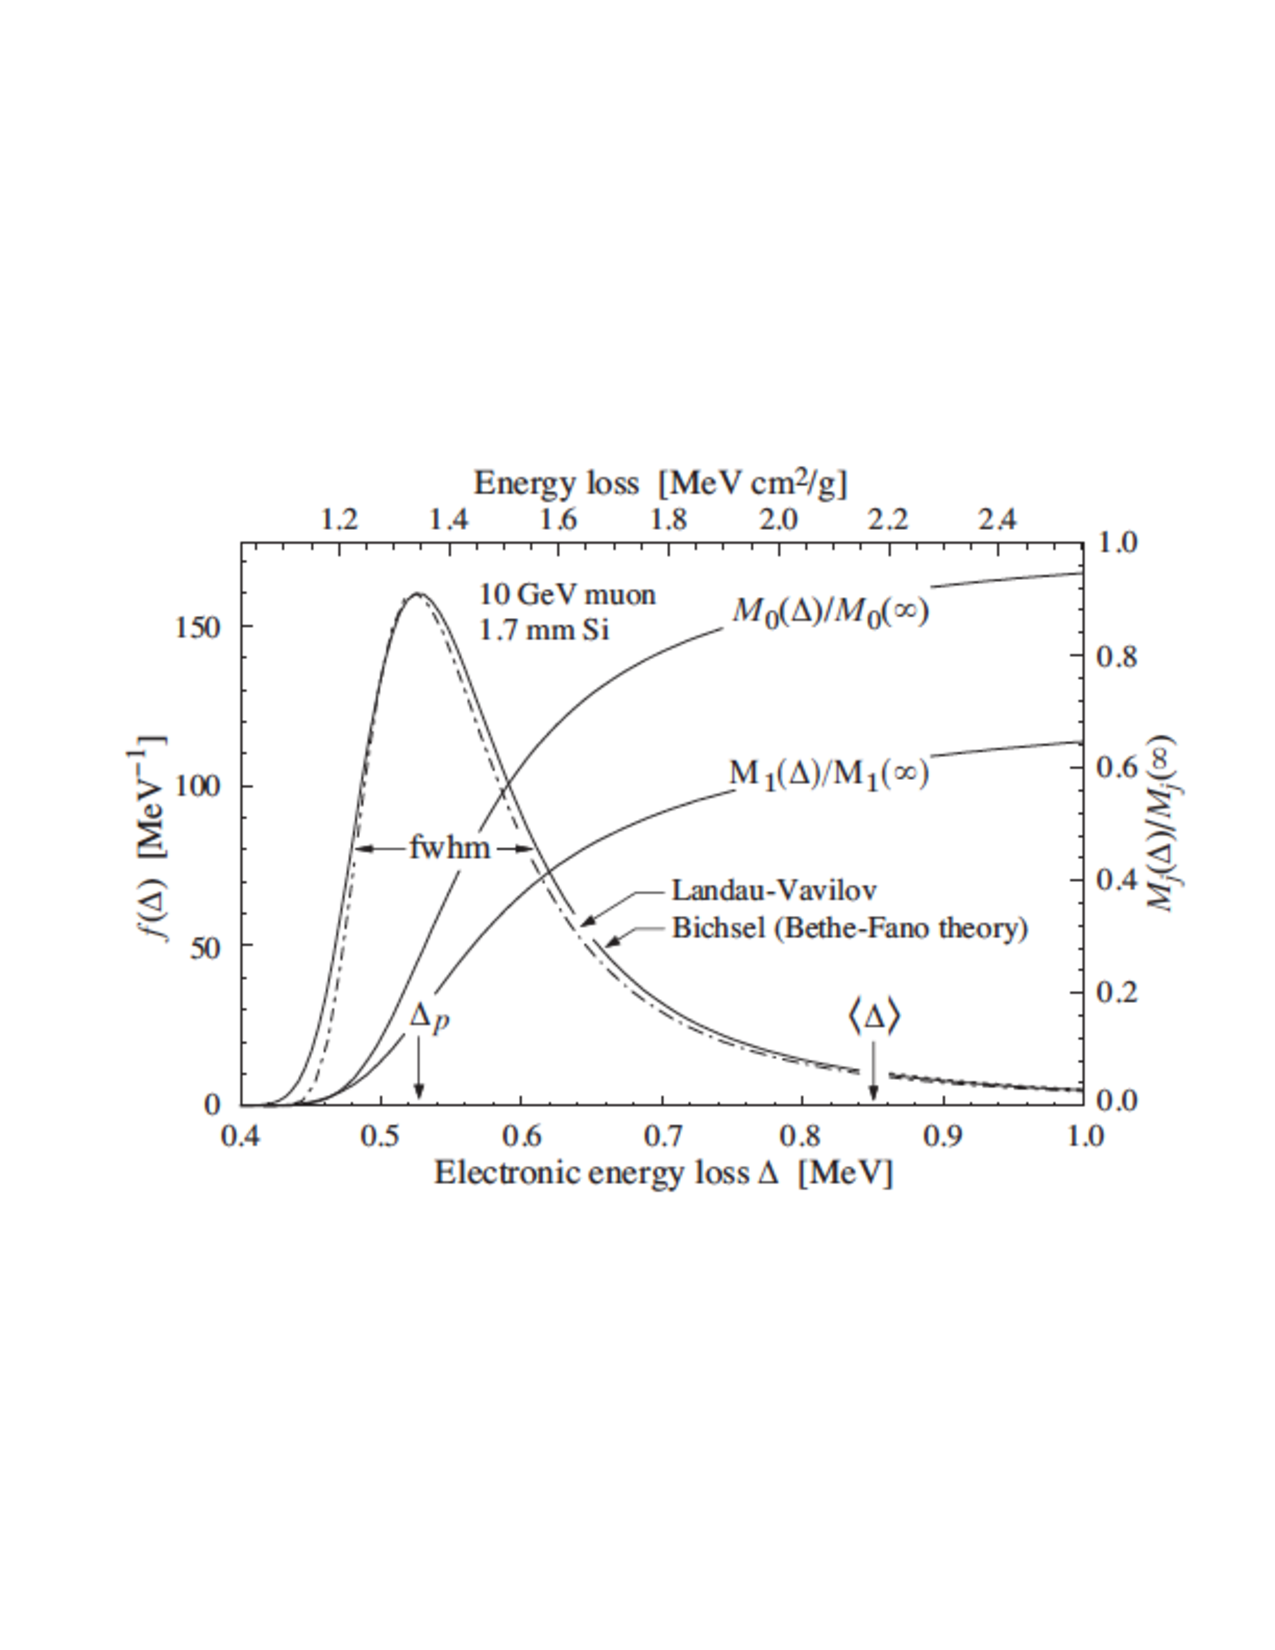
\includegraphics[scale=0.5]{./particleinteractions/Pictures/landau.pdf}
\caption{Stolen from the particle data group, this picture shows the distribution of energy deposits for a 10 GeV muon transversing 1.7 mm of silicon. }
\label{fig:landau}
\end{figure}

Sometimes a particle passes close enough to an atom to interact with the nucleus, instead of the electrons.  The mass of the nucleus, and the force binding it into its places in the crystal lattice, are large compared to the mass of the particle.  The particle usually bounces off the nucleus the way a ball bounces off a wall, changing direction, but without losing energy.  For a material that is not very thin, this can happen multiple times, and thus this is called "multiple scattering".  Fig~\ref{fig:pdgmultscattcartoon} shows a cartoon of this process.


\begin{figure}[h]
\centering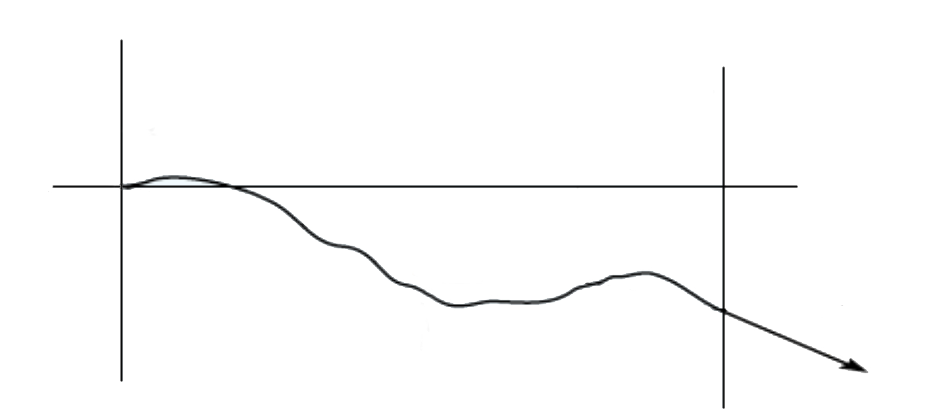
\includegraphics[scale=0.5]{./particleinteractions/Pictures/multscattcartoon.pdf}
\caption{Stolen from the particle data group, this picture shows a cartoon showing the path of a charged particle undergoing multiple scattering in matter }
\label{fig:pdgmultscattcartoon}
\end{figure}



\section{Interactions of gamma rays with matter}\index{gammainteractions}

Here we call them “gamma rays” instead of photons because we are going to discuss only those photons of interest to particle physics: ones with energies above a keV or so.

There are several ways a gamma ray can interaction with matter:
\begin{itemize}
\item photoelectric effect
\item Compton scattering
\item pair production in the field of the nucleus
\item pair production in the field of the electron
\item photonuclear interactions
\end{itemize}

The photoelectric effect was very important in the development of quantum mechanics.  Einstein was awarded the Nobel Prize for his work on its understanding.  It is an interaction between a photon and an atom electron.  If the photon has energy greater than the binding energy of the electron to the atom, it can eject the electron.  The electron will have a kinetic energy equal to the energy of the photon minus the binding energy.


Compton scatting is scatting of a photon off an electron.  The Feynman diagram is shown in Figure ~\ref{fig:compton}. 


\begin{figure}[h]
\centering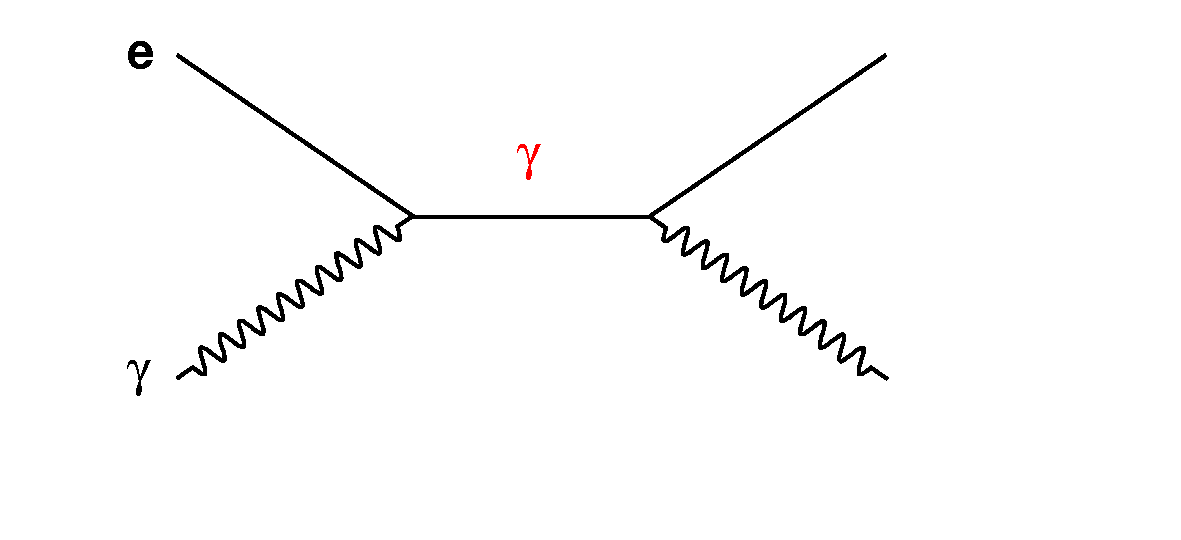
\includegraphics[scale=0.5]{./particleinteractions/Pictures/compton.pdf}
\caption{Feynmann diagram for Compton scattering of a photon by an electron}
\label{fig:compton}
\end{figure}

Pair production is the conversion of a photon into an electron-position pair through an interaction (usually) with a nucleus.  The Feynmann diagram is shown below.


\begin{figure}[h]
\centering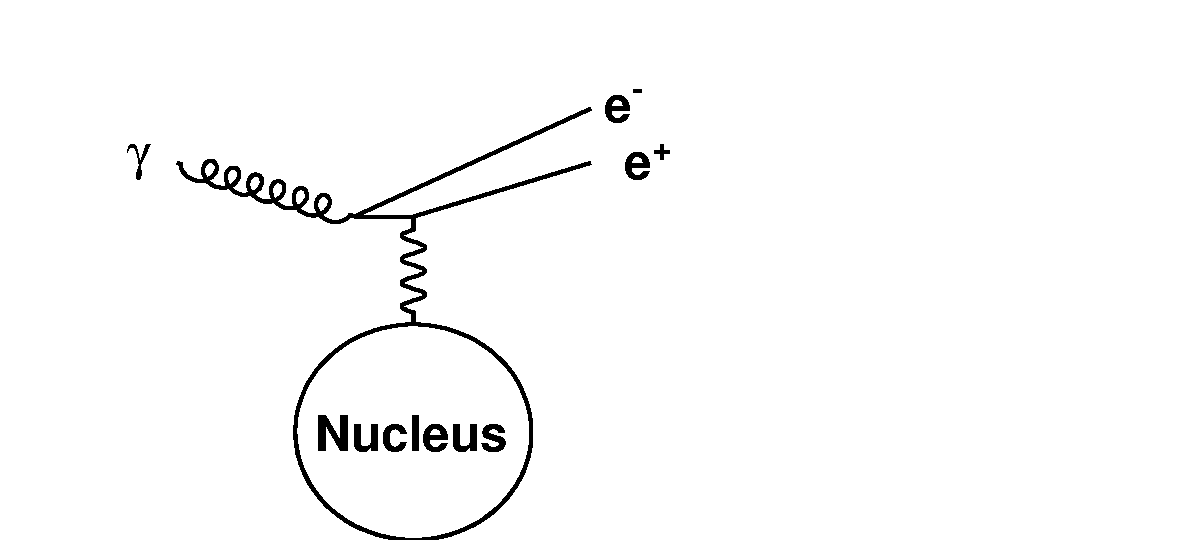
\includegraphics[scale=0.5]{./particleinteractions/Pictures/pairproduction.pdf}
\caption{Feynmann diagram for pair production in the field of a nucleus}
\label{fig:pairproduction}
\end{figure}



Figure~\ref{fig:photoninteractions} shows the cross section for each mechanism as a 
function of photon energy.  As you can see, for photons with energy greater than twice the 
electron mass, pair production is the most important mechanism.  We will discuss this in more detail when we discuss calorimetry.


\begin{figure}[h]
\centering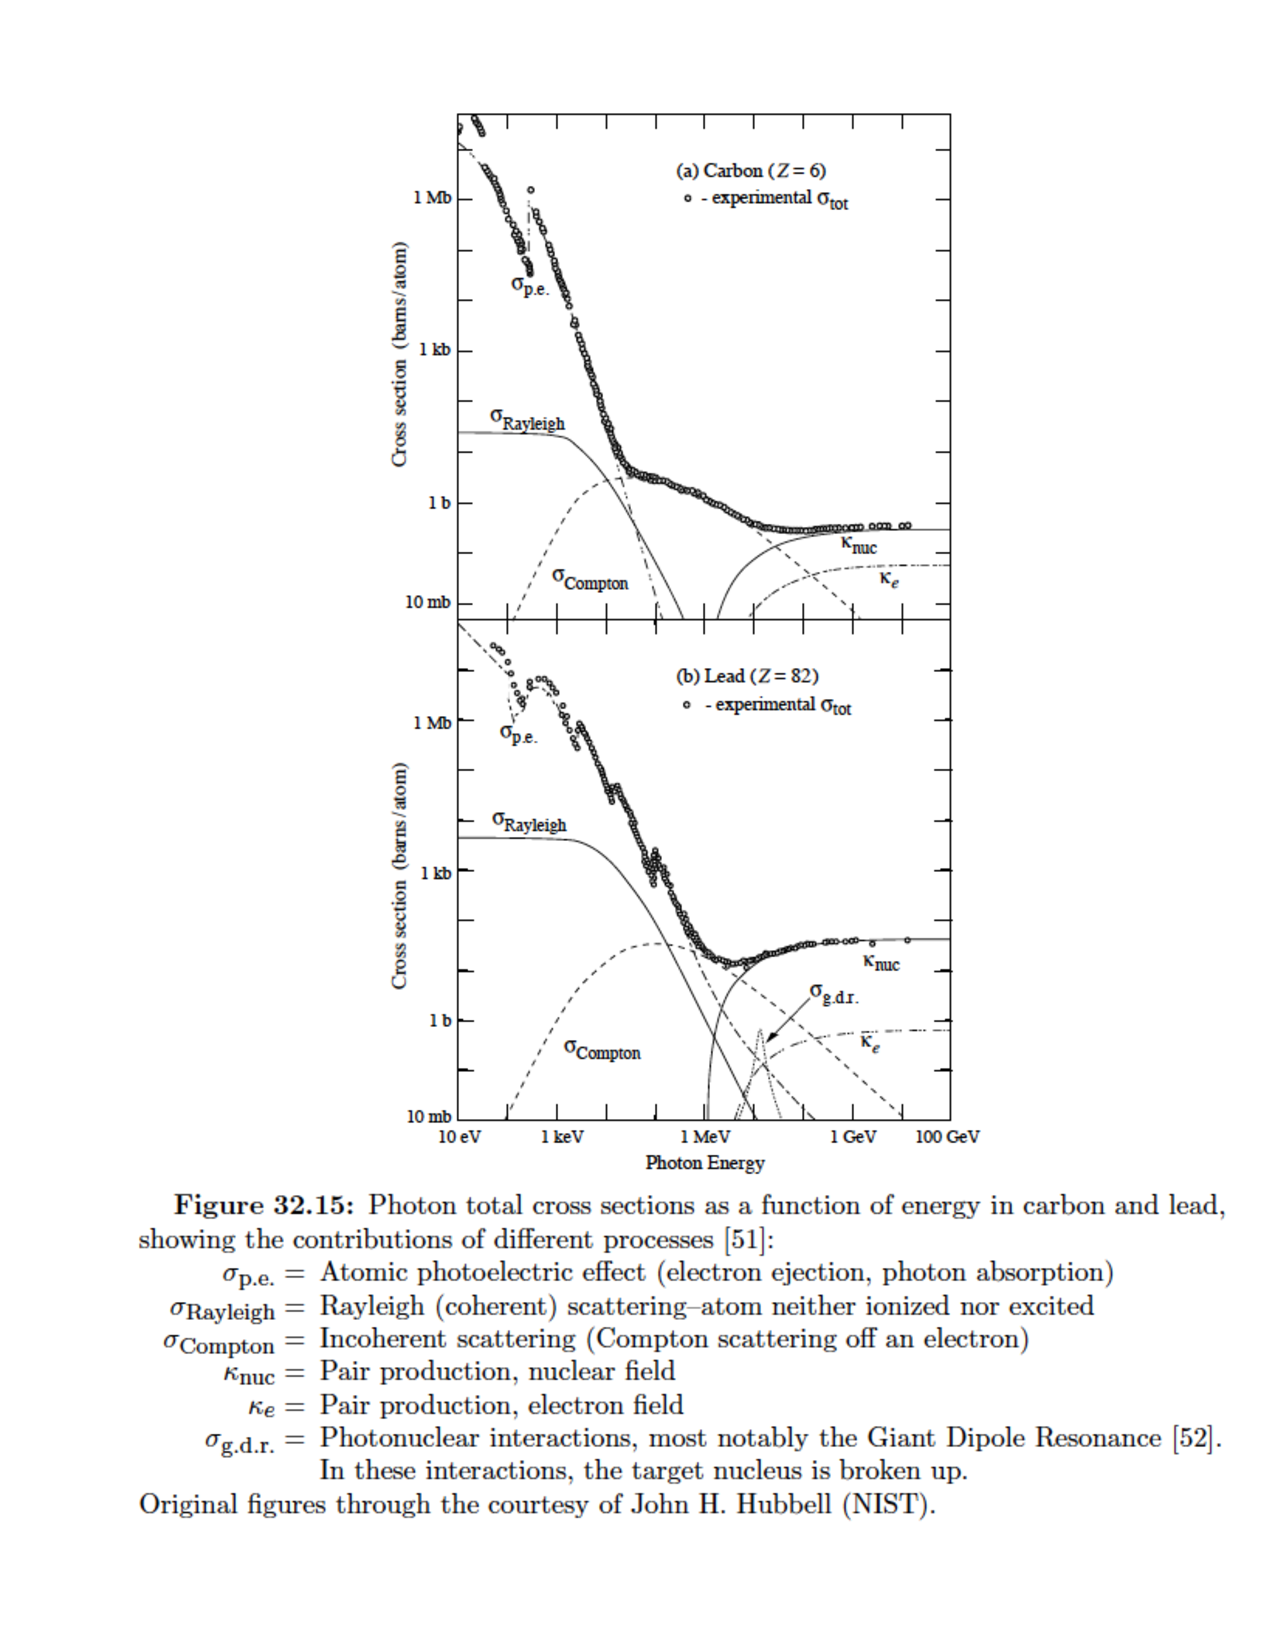
\includegraphics[scale=0.5]{./particleinteractions/Pictures/photoninteractions.pdf}
\caption{Stolen from the particle data group, this picture shows the cross sections for possible interactions of photons with matter as a function of photon energy }
\label{fig:photoninteractions}
\end{figure}

